\documentclass{beamer}
\usepackage{url}
\usetheme{Berlin}
\definecolor{UBCblue}{rgb}{0.04706, 0.13725, 0.26667} % UBC Blue (primary)

\definecolor{UCBblue}{rgb}{0.09706, 0.2725, 0.46667} % UBC 
\usecolortheme[named=UBCblue]{structure}
\title{Understanding \textbf{TV Transmitter Antennas}: Types and Characteristics}

\author{Adhithya S}

\date{February 7, 2023}

\begin{document}

\frame{\titlepage}

\section{Introduction}


\begin{frame}
  \frametitle{Introduction}
  \begin{block}{What is an Antenna?}
    An antenna is a device that converts electrical energy into electromagnetic (EM) waves, and vice versa.
  \end{block}
  \pause
  \begin{block}{Analogy with a Light Bulb}
    Just as a light bulb converts electrical energy into light, an antenna converts electrical energy into EM waves.
  \end{block}
\end{frame}

\section{Antenna Principle}

\begin{frame}
\frametitle{General Antenna Working}
\begin{itemize}
\item An electric signal is converted to an Electromagnetic wave.

\item An Electromagnetic wave is a combination of an electric and magnetic field. Energy transfer requires both fields.
\pause

\item How to make electric or magnetic field leave the conductor? 

\pause

\item To make the electric field move, a dipole with two opposite charges separated by a distance is used. Moving the dipole quickly distorts the electric field and creates a \textbf{kink}, which cuts off the electric field from the wire and propagates at the speed of light.
\end{itemize}
\end{frame}

\begin{frame}
\frametitle{Antenna Working Principle (Continued)}
    \begin{itemize}
        \item The propagated electric field generates a perpendicular magnetic field.
        
        \pause
        
        \item The magnetic field generates an electric field, creating a cycle until the energy of the wave decreases and disperses into space.
    \end{itemize}
\end{frame}


\begin{frame}
  \frametitle{Types of Antennas}
  \begin{block}{Omnidirectional Antennas}

    Omnidirectional antennas emit EM waves in all directions. They are often used for simple wireless communication systems, such as Wi-Fi.
  \end{block}
  \begin{block}{Directional Antennas}

    Directional antennas emit EM waves in a specific direction. They are often used for more complex wireless communication systems, such as satellite communication.
  \end{block}
\end{frame}




\section{Antennas Types}

\subsection{Dipole Antenna}
\begin{frame}
    \frametitle{Explanation of How a Dipole Antenna Works}
    A dipole antenna consists of two metal elements that are equal in length and mounted perpendicular to each other. The dipole antenna transmits the signal in all directions, creating an omnidirectional pattern.
    \begin{center}
        
    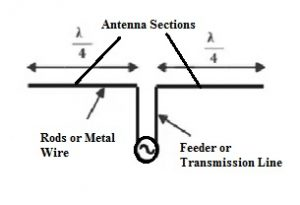
\includegraphics[width=3in]{dipole.jpg}
    \end{center}
\end{frame}

\begin{frame}
\frametitle{Explanation of How a Room Lamp Illuminates in All Directions and Comparison to Dipole Antenna}


A room lamp illuminates in all directions by emitting light in all directions.

Similarly, a dipole antenna transmits broadcast in all directions by emitting the signal in all directions, creating an omnidirectional pattern.


        \begin{figure}[htbp]
        \begin{minipage}[b]{0.5\linewidth}
            \centering
            
\includegraphics[width=0.8\linewidth]{bulb.jpg}
    
            \end{minipage}%
            \begin{minipage}[b]{0.5\linewidth}
            \centering
            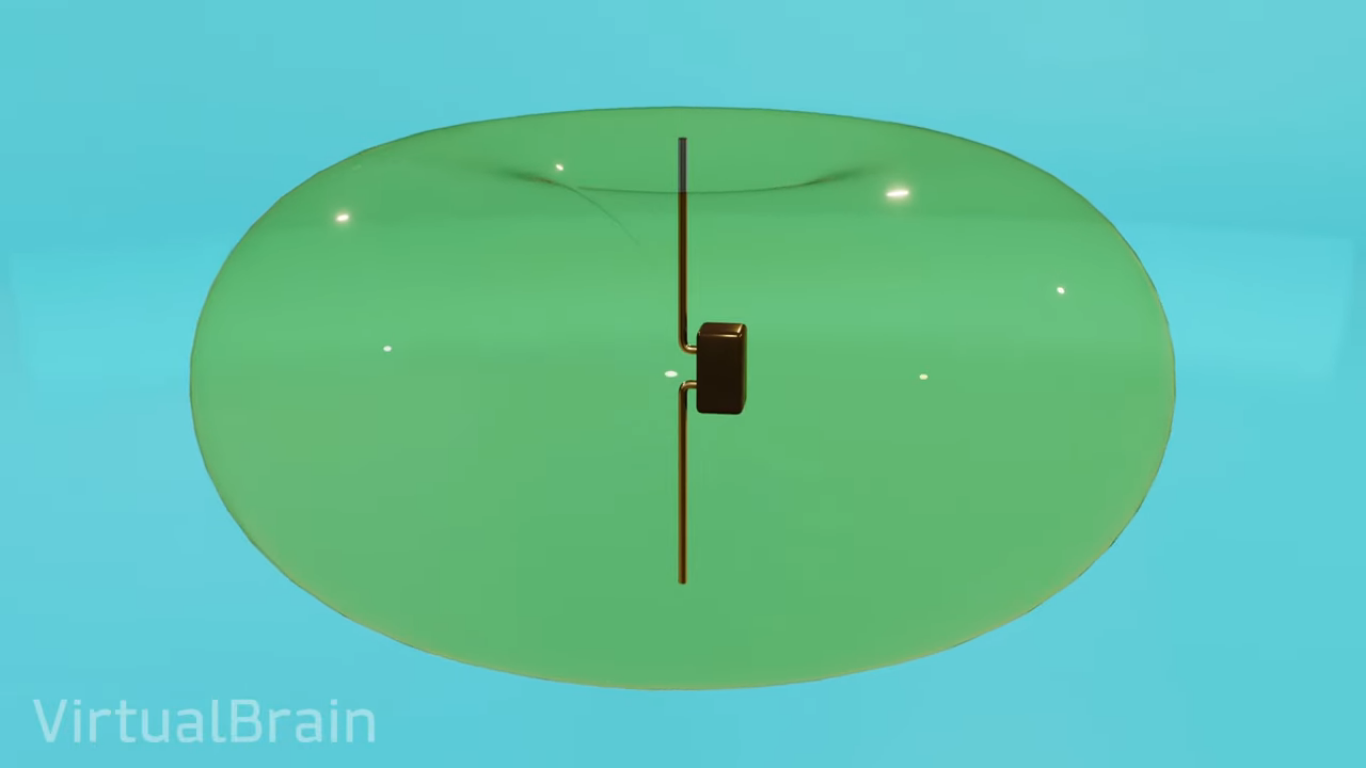
\includegraphics[width=0.8\linewidth]{diprad.png}
        \end{minipage}
        \end{figure}

\end{frame}


\subsection{Yagi Antenna}

\begin{frame}
    \frametitle{Explanation of How a Yagi Antenna Works}
    A Yagi antenna is a type of directional antenna that uses a series of parallel metal elements to focus the transmission in one direction.


        \begin{figure}[htbp]
        \begin{minipage}[b]{0.5\linewidth}
            \centering
            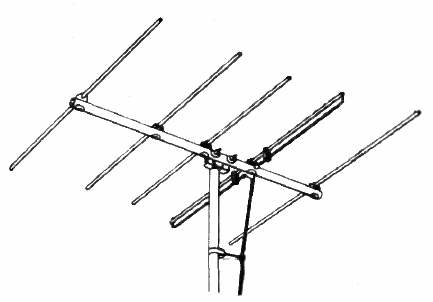
\includegraphics[width=0.8\linewidth]{yagi.png}
            \pause
            
            \end{minipage}%
            \begin{minipage}[b]{0.5\linewidth}
            \centering
            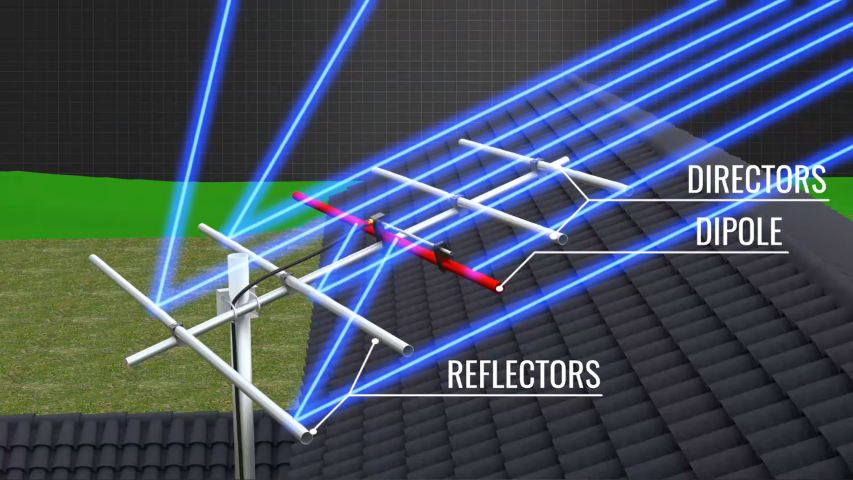
\includegraphics[width=0.8\linewidth]{yagibeam.png}
        \end{minipage}
        \end{figure}
        
\end{frame}

\begin{frame}
    \frametitle{Characteristics: Directional, Long-Range Transmission}
    Yagi antennas are directional, meaning they transmit the signal in one specific direction. This allows for long-range transmission, as the energy is focused in a specific direction instead of being scattered in all directions.
        \begin{figure}[htbp]
           \begin{minipage}[b]{0.5\linewidth}
            \centering
            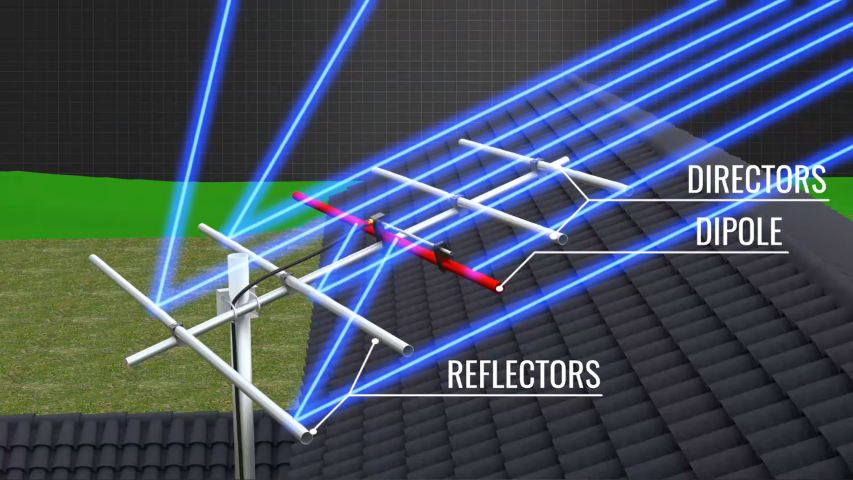
\includegraphics[width=0.8\linewidth]{yagibeam.png}
        \end{minipage}
        \end{figure}
        
\end{frame}


\subsection{Patch Antenna}

\begin{frame}
    \frametitle{Explanation of How a Patch Antenna Works}
    A patch antenna is a type of directional antenna that uses a flat metal element to transmit the signal in one specific direction. The signal is then focused in a specific area, allowing for short-range transmission.
        \begin{center}
        
    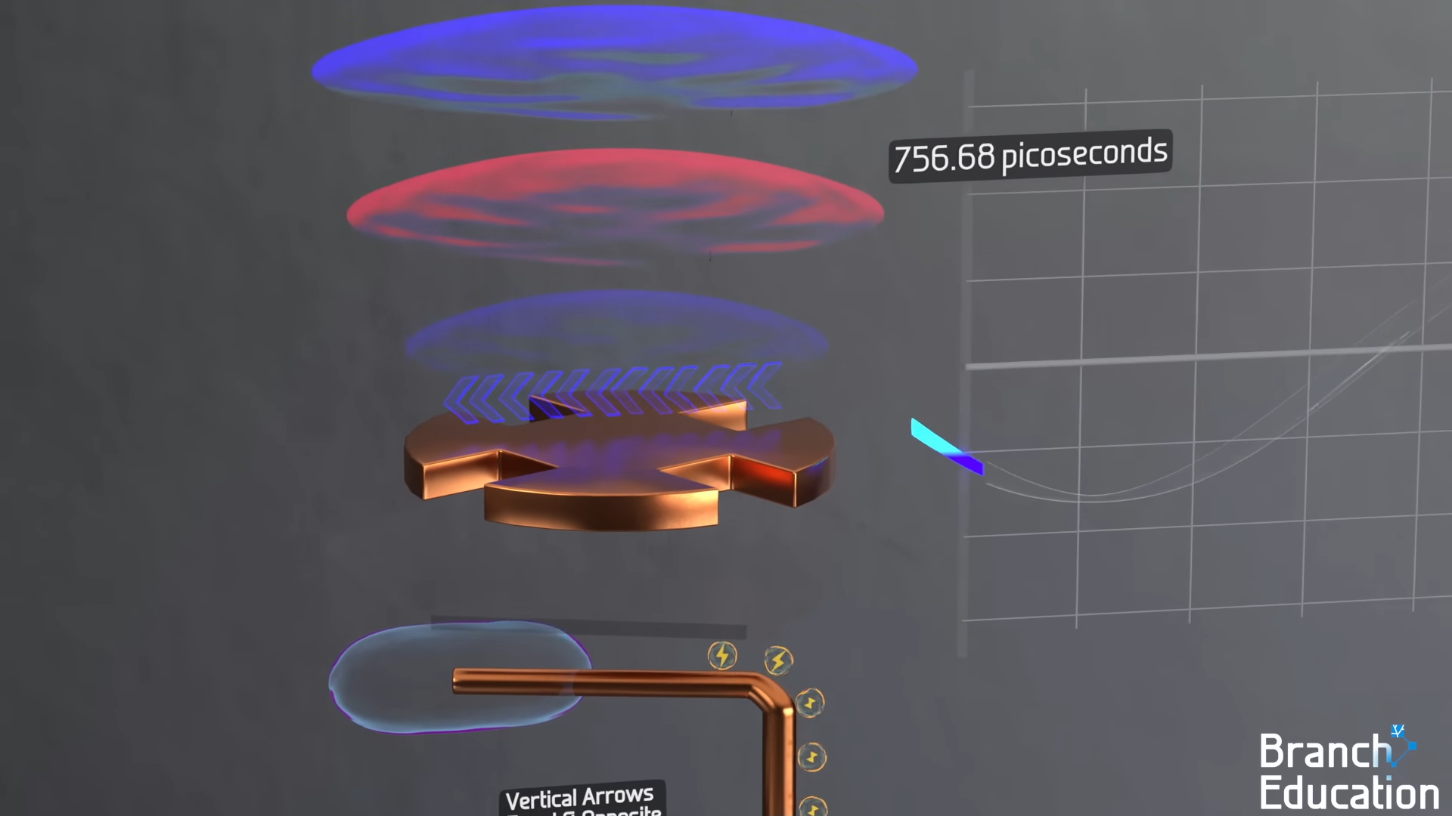
\includegraphics[width=3in]{patch2.png}
    \end{center}
\end{frame}

\begin{frame}
\frametitle{Explanation of How a Magnifying Glass Focuses Light and Comparison to a Patch Antenna}

A magnifying glass focuses light in a specific area by using a lens to direct the light as a beam.


Similarly, a patch antenna focuses broadcast transmission using flat metal element to direct the energy as a beam.

        \begin{figure}[htbp]
        \begin{minipage}[b]{0.5\linewidth}
            \centering
            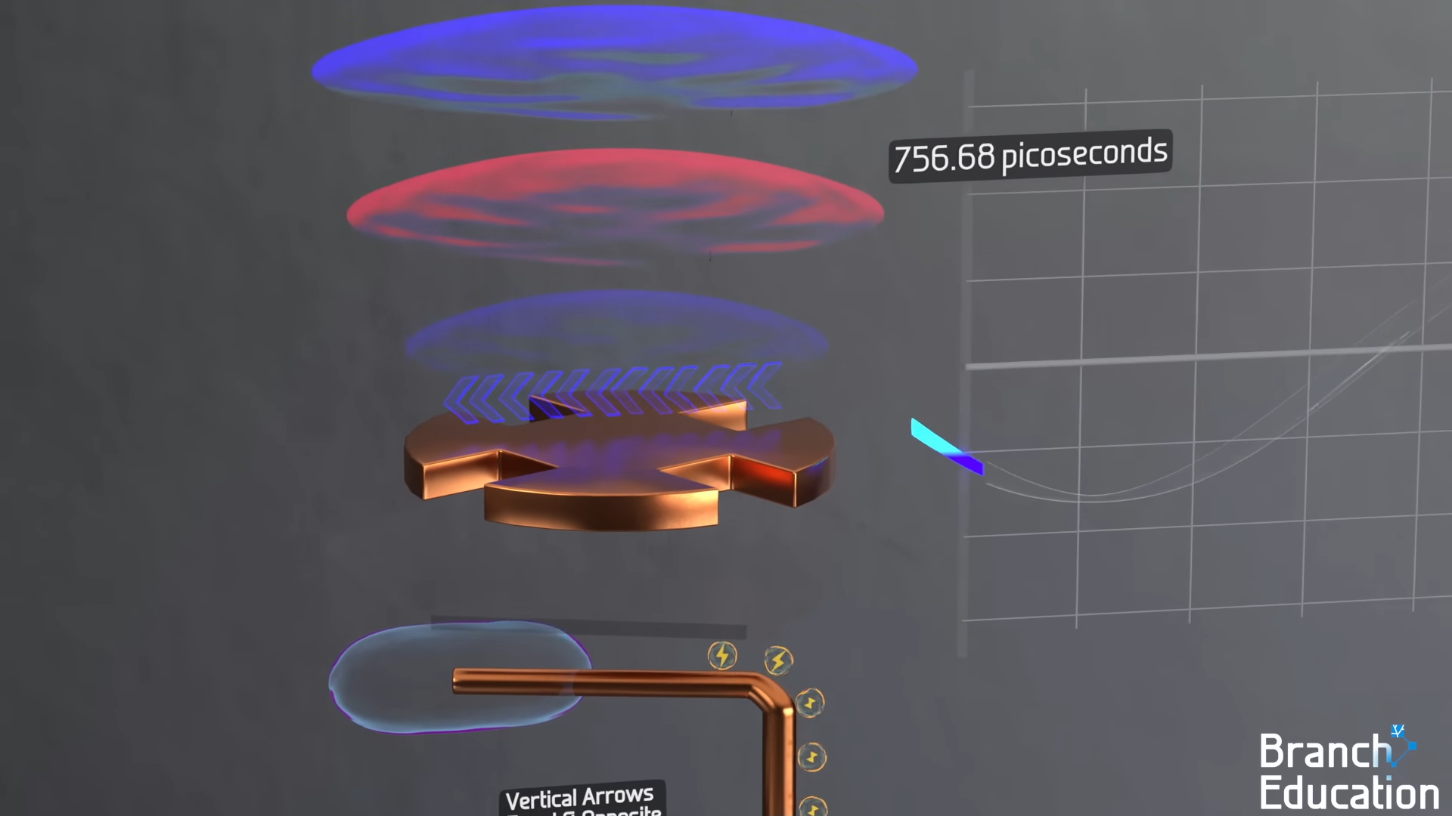
\includegraphics[width=0.8\linewidth]{patch2.png}
            \end{minipage}%
            \begin{minipage}[b]{0.5\linewidth}
            \centering
            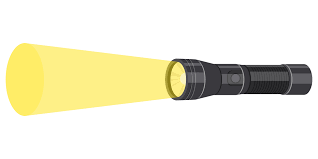
\includegraphics[width=0.8\linewidth]{flashlight.png}
        \end{minipage}
        \end{figure}
\end{frame}

\section{Conclusion}

\begin{frame}
\frametitle{Recap}
In this presentation, we have reviewed.

\begin{itemize}
    \item \textbf{Types} of TV transmitter antennas 
    \begin{itemize}
        \item Yagi
        \item Patch
        \item Diopole
    \end{itemize}
    \item Discussed their respective \textbf{characteristics} i.e. Their Radiation pattern.
    
\end{itemize}


\end{frame}

\begin{frame}{Acknowledgements \& Doubts? \& Thank You}
    \begin{itemize}
        \item Presentation Made with \LaTeX Beamer package, Source code available \href{https://airgapflux.co.in/?search=Antenna&subject=coel&restype=0}{\color{UCBblue}{\textbf{here}}}
        \item Base template Presentation code and basic content by {\color{UCBblue}{\textbf{ChatGPT}}}
        \item Adobe Photoshop - Kink progression.        
        \item Dipole antenna Radiation - Comsol
        \item  Theory learnt from multiple sources listed \href{https://airgapflux.co.in/?search=Antenna&subject=coel&restype=0}{\color{UCBblue}{\textbf{here}}}
    \end{itemize}
\end{frame}
\end{document}